% Recurrent Minds -- CSE638 CT1 Task 3 paper (IEEEtran journal format).
% Build:  tectonic journal.tex   (clean journal version)
%         tectonic ct1_submission.tex   (same paper with the designed course cover page)
% All numbers come from generated/macros.tex and generated/tab_*.tex (python build_latex.py).
\documentclass[journal,a4paper]{IEEEtran}
\usepackage[T1]{fontenc}
\usepackage{amsmath,amssymb}
\usepackage{graphicx}
\usepackage{booktabs}
\usepackage{multirow}
\usepackage{adjustbox}
\newcommand{\fittable}[1]{\begin{adjustbox}{max width=\columnwidth}\input{#1}\end{adjustbox}}
\usepackage{xcolor}
\usepackage{tikz}
\usepackage{cite}
\usepackage[hidelinks]{hyperref}
\usepackage{url}
\graphicspath{{figures/}{../../results/figures/}{../}}
% generated by build_latex.py -- do not edit
\newcommand{\bestbpc}{1.498}
\newcommand{\bestppl}{2.824}
\newcommand{\bestval}{1.519}
\newcommand{\br}{0.80}
\newcommand{\bunit}{112}
\newcommand{\finepochs}{18.0}
\newcommand{\fingain}{0.087}
\newcommand{\finmin}{91}
\newcommand{\finratio}{3.2}
\newcommand{\finsteps}{8{,}000}
\newcommand{\finvsng}{9.4}
\newcommand{\greedydtwo}{0.177}
\newcommand{\greedynll}{0.832}
\newcommand{\greedyrep}{78}
\newcommand{\gruvsng}{4.1}
\newcommand{\interpchars}{60{,}000}
\newcommand{\mingru}{45.4}
\newcommand{\minhlarge}{83.6}
\newcommand{\minhsmall}{19.5}
\newcommand{\minlone}{25.3}
\newcommand{\minlstm}{36.9}
\newcommand{\minlthree}{71.0}
\newcommand{\minrnn}{20.5}
\newcommand{\minseqA}{33.0}
\newcommand{\minseqB}{43.2}
\newcommand{\minseqD}{56.1}
\newcommand{\ngctxfive}{197}
\newcommand{\ngfive}{1.653}
\newcommand{\ngpplfive}{3.145}
\newcommand{\ngpplseven}{3.256}
\newcommand{\ngpplthree}{4.163}
\newcommand{\ngseven}{1.703}
\newcommand{\ngthree}{2.058}
\newcommand{\ngvalfive}{1.681}
\newcommand{\ngvalseven}{1.747}
\newcommand{\ngvalthree}{2.078}
\newcommand{\nucdtwo}{0.958}
\newcommand{\nucvalid}{97.1}
\newcommand{\paramsGRU}{666{,}123}
\newcommand{\paramsLSTM}{880{,}139}
\newcommand{\paramsRNN}{238{,}091}
\newcommand{\pargru}{0.666}
\newcommand{\parhlarge}{1.908}
\newcommand{\parhsmall}{0.246}
\newcommand{\parlone}{0.354}
\newcommand{\parlstm}{0.88}
\newcommand{\parlthree}{1.406}
\newcommand{\parrnn}{0.238}
\newcommand{\parseqA}{0.88}
\newcommand{\parseqB}{0.88}
\newcommand{\parseqD}{0.88}
\newcommand{\pplgru}{3.000}
\newcommand{\pplhlarge}{3.030}
\newcommand{\pplhsmall}{4.075}
\newcommand{\ppllone}{3.555}
\newcommand{\ppllstm}{3.308}
\newcommand{\ppllthree}{3.525}
\newcommand{\pplrnn}{3.401}
\newcommand{\pplseqA}{3.332}
\newcommand{\pplseqB}{3.320}
\newcommand{\pplseqD}{3.295}
\newcommand{\qacc}{89.0}
\newcommand{\qacccur}{53.5}
\newcommand{\qmaj}{57.0}
\newcommand{\qr}{0.90}
\newcommand{\qunit}{201}
\newcommand{\rawchars}{4.18}
\newcommand{\refvalid}{99.7}
\newcommand{\tbpcgru}{1.585}
\newcommand{\tbpchlarge}{1.599}
\newcommand{\tbpchsmall}{2.027}
\newcommand{\tbpclone}{1.830}
\newcommand{\tbpclstm}{1.726}
\newcommand{\tbpclthree}{1.818}
\newcommand{\tbpcrnn}{1.766}
\newcommand{\tbpcseqA}{1.736}
\newcommand{\tbpcseqB}{1.731}
\newcommand{\tbpcseqD}{1.720}
\newcommand{\testchars}{202{,}384}
\newcommand{\tfivedone}{0.507}
\newcommand{\tfivevalid}{99.6}
\newcommand{\thirteenvalid}{74.4}
\newcommand{\tonedone}{0.671}
\newcommand{\tonevalid}{90.0}
\newcommand{\totchars}{4.05}
\newcommand{\totwords}{731}
\newcommand{\trainchars}{3{,}642{,}687}
\newcommand{\unigramH}{4.411}
\newcommand{\unigramPPL}{21.27}
\newcommand{\unseeneight}{16.3}
\newcommand{\unseenfive}{1.4}
\newcommand{\unseenseven}{8.8}
\newcommand{\unseenten}{36.7}
\newcommand{\valchars}{202{,}381}
\newcommand{\vbpcgru}{1.611}
\newcommand{\vbpchlarge}{1.623}
\newcommand{\vbpchsmall}{2.047}
\newcommand{\vbpclone}{1.851}
\newcommand{\vbpclstm}{1.752}
\newcommand{\vbpclthree}{1.843}
\newcommand{\vbpcrnn}{1.791}
\newcommand{\vbpcseqA}{1.761}
\newcommand{\vbpcseqB}{1.757}
\newcommand{\vbpcseqD}{1.747}
\newcommand{\vocab}{75}
\newcommand{\wordrtwo}{0.82}
\newcommand{\wordrtwocur}{0.42}

\newcommand{\BPC}{\mathrm{BPC}}
\hyphenation{Witten Bell Gutenberg Austen}

\begin{document}

\ifdefined\WITHCOVER
\thispagestyle{empty}
\begin{tikzpicture}[remember picture,overlay]
  \node at (current page.center) {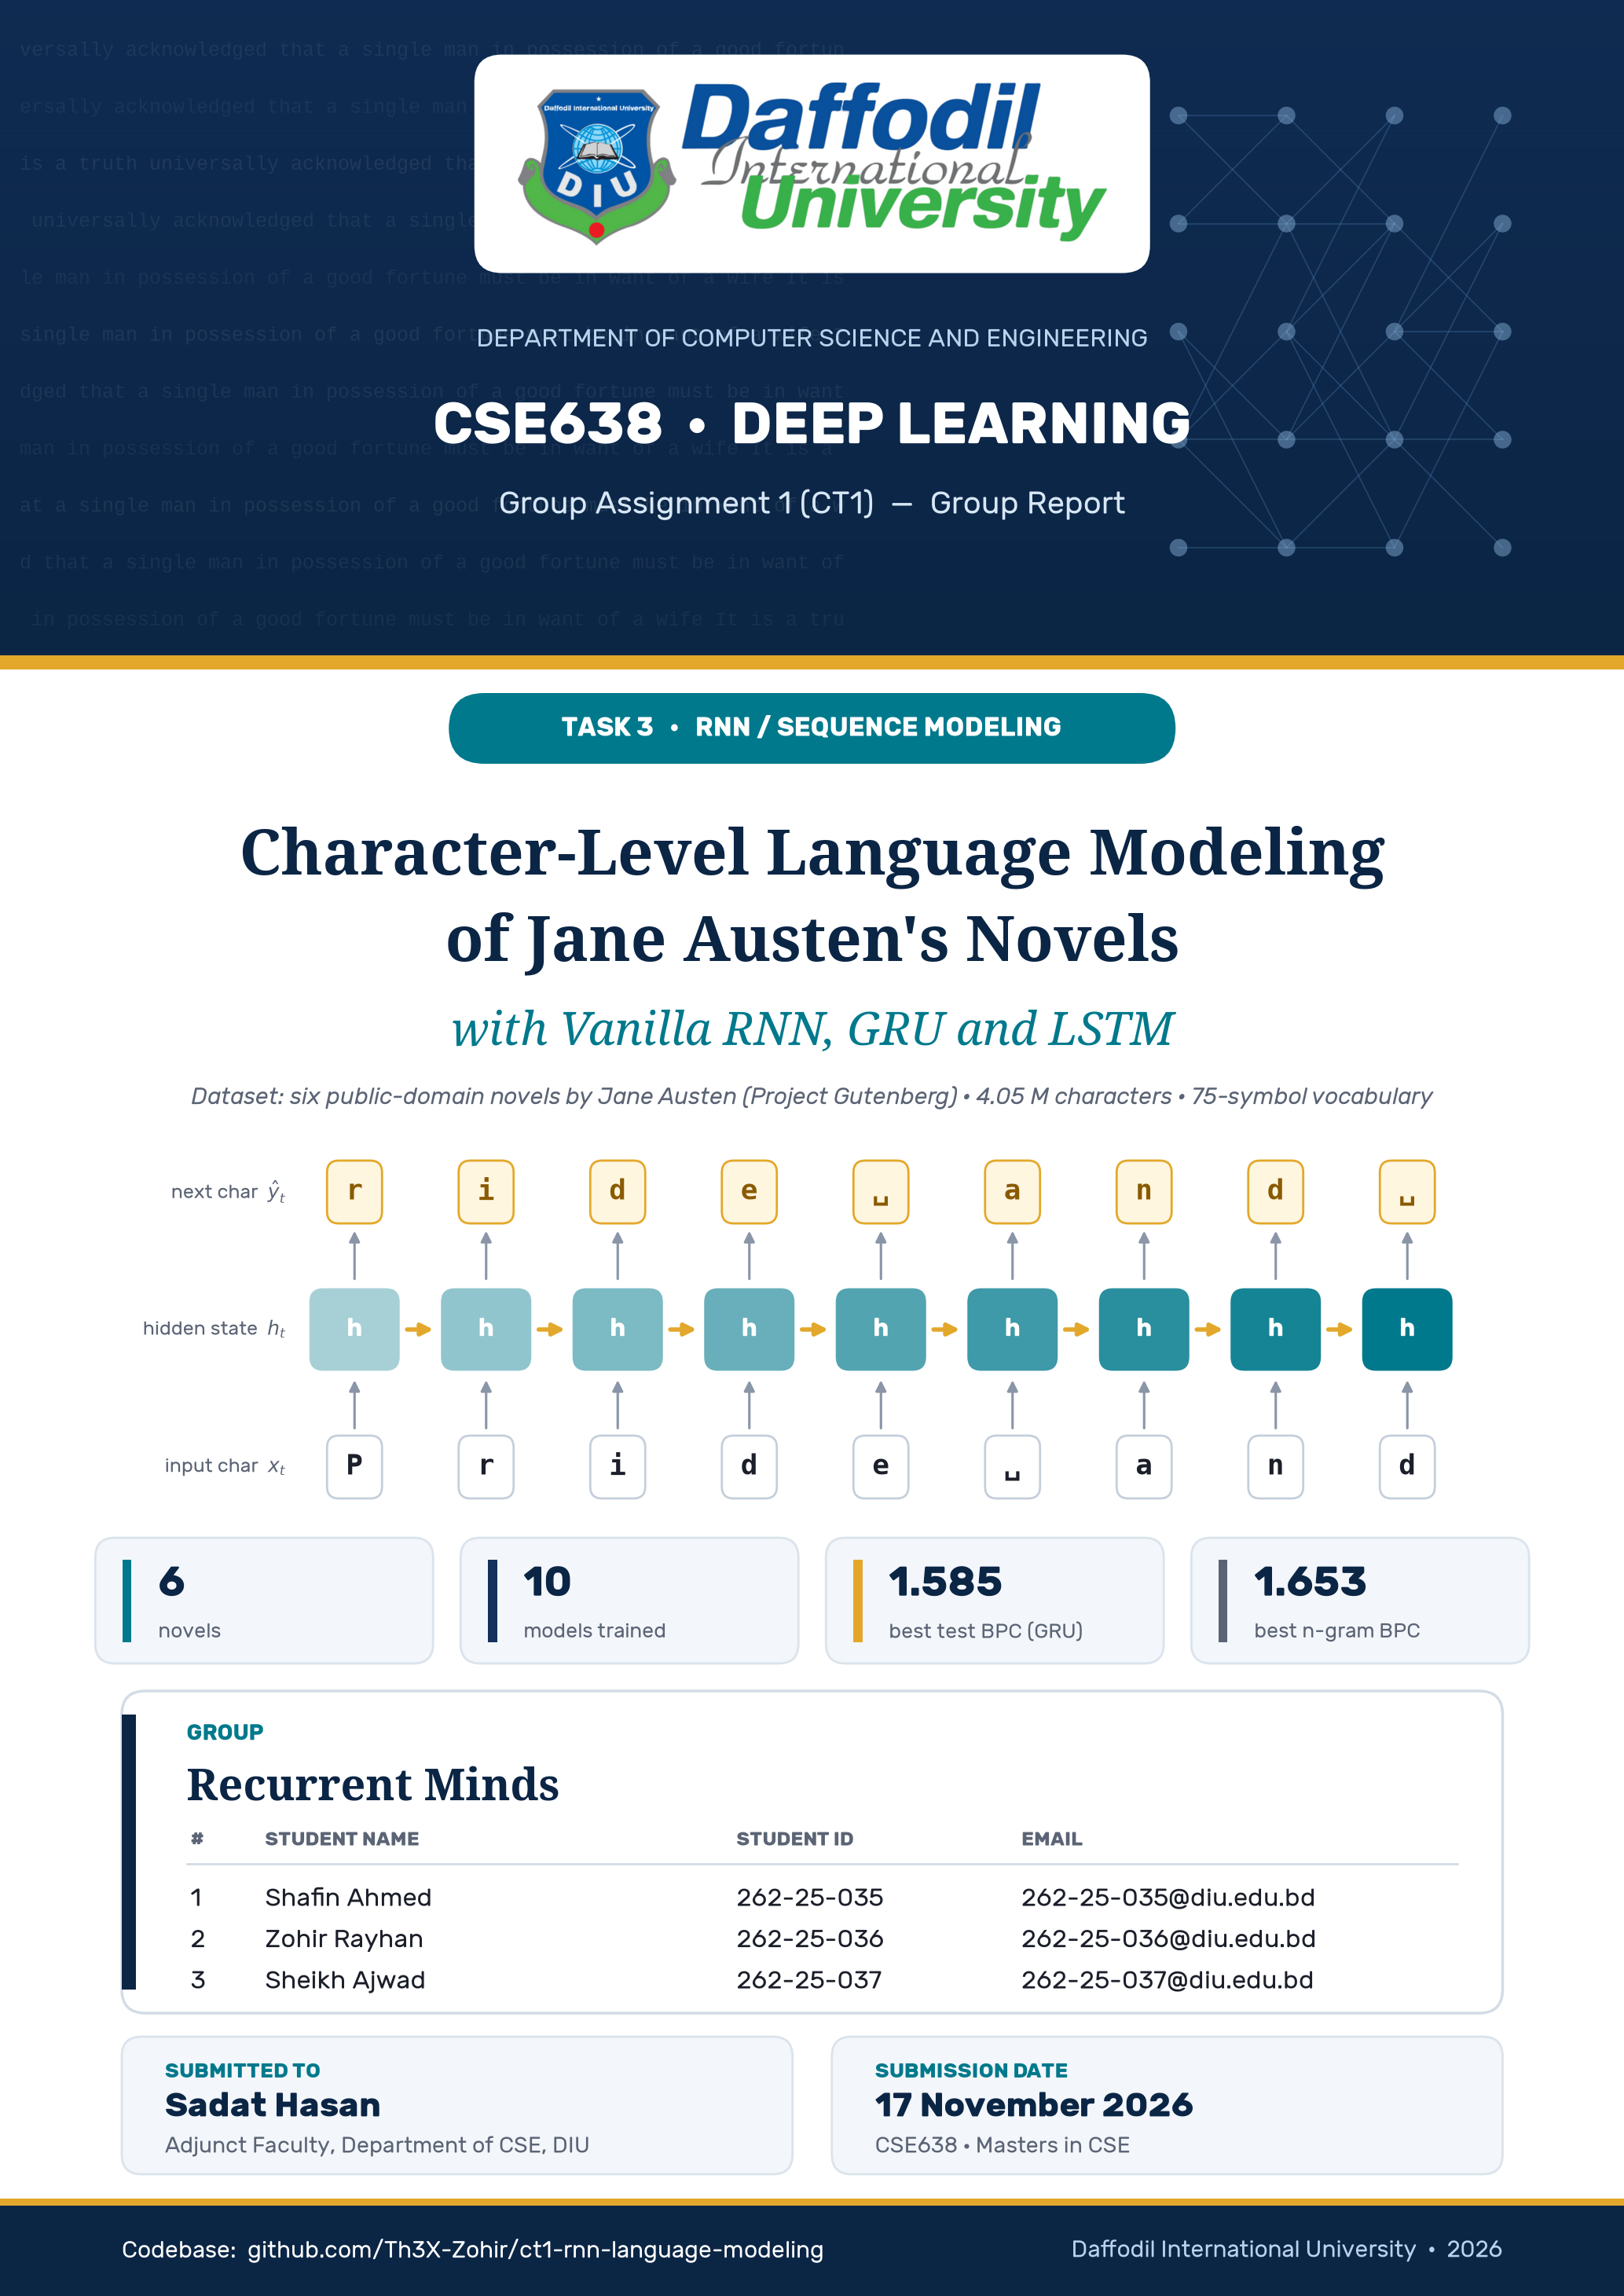
\includegraphics[width=\paperwidth,height=\paperheight]{cover_page.png}};
\end{tikzpicture}
\null\clearpage
\setcounter{page}{1}
\fi

\title{Character-Level Language Modeling of Jane Austen's Novels: A Controlled Comparison of Vanilla RNN, GRU and LSTM Networks}

\author{Shafin~Ahmed,~Zohir~Rayhan,~and~Sheikh~Ajwad%
\thanks{The authors are with the Department of Computer Science and Engineering, Daffodil International University, Dhaka, Bangladesh (e-mail: 262-25-035@diu.edu.bd; 262-25-036@diu.edu.bd; 262-25-037@diu.edu.bd).}%
\thanks{Group Assignment~1 (CT1), CSE638 Deep Learning, submitted to Sadat Hasan, Adjunct Faculty. Code, data pipeline and trained models: \url{https://github.com/Th3X-Zohir/ct1-rnn-language-modeling}.}}

\markboth{CSE638 Deep Learning, Group Assignment 1 (CT1), November 2026}%
{Ahmed \MakeLowercase{\textit{et al.}}: Character-Level Language Modeling with RNN, GRU and LSTM}

\maketitle

\begin{abstract}
We study character-level language modeling on six novels by Jane Austen (\totchars~M characters, a \vocab-symbol vocabulary) and ask which design choices of a recurrent network actually matter. Ten models were trained under an identical budget of 2{,}500 updates: a vanilla RNN, a GRU and an LSTM of the same width, the LSTM with four truncated back-propagation lengths, and the LSTM with five capacities. They are compared against interpolated Witten--Bell $n$-gram models, and seven decoding strategies are evaluated on generated text. Under the equal budget the GRU learns fastest and reaches \tbpcgru~bits per character (BPC) on held-out text, ahead of the LSTM (\tbpclstm) and the vanilla RNN (\tbpcrnn). Hidden size and gating matter far more than the BPTT window, which changes the result by less than 0.02~BPC. A 5-gram model is a surprisingly strong baseline (\ngfive~BPC) that only the gated networks beat. Training the best configuration \finratio$\times$ longer lowers the test score to \bestbpc~BPC (perplexity \bestppl). Probing the hidden state shows that a single unit has learned to track whether the text is inside a quotation, information a linear probe recovers with \qacc\% accuracy against \qacccur\% from the current character alone. Nucleus sampling gives the best balance between correct spelling and diversity, while greedy decoding quickly falls into loops. The trained model also runs in an in-browser demo written in plain JavaScript.
\end{abstract}

\begin{IEEEkeywords}
Recurrent neural networks, LSTM, GRU, character-level language model, bits per character, text generation, decoding strategies, interpretability.
\end{IEEEkeywords}

\section{Introduction}
\IEEEPARstart{A}{} language model assigns a probability to the next symbol given everything before it. That single ability underlies autocompletion, speech recognition, machine translation and, at very large scale, today's chat assistants. Before attention-based models became standard, recurrent neural networks (RNNs) were the default tool for the job: they read a sequence one step at a time and carry a hidden state that summarises what they have seen so far~\cite{elman1990}.

Plain RNNs are hard to train over long spans because gradients shrink or explode as they are multiplied through many time steps~\cite{bengio1994,pascanu2013}. Gated cells were designed to fix this. The long short-term memory (LSTM)~\cite{hochreiter1997lstm} adds a separate cell state that is updated additively, and the gated recurrent unit (GRU)~\cite{cho2014gru} reaches a similar effect with fewer gates. Which of them works better is still debated, and the answer depends heavily on the task and on how long the models are trained~\cite{chung2014,jozefowicz2015}.

This paper addresses Task~3 of our course assignment, recurrent sequence modeling, using a character-level formulation. Characters keep the vocabulary tiny (\vocab~symbols), remove the out-of-vocabulary problem, and force the model to learn spelling, punctuation and grammar from scratch, so differences between cells show up clearly. We use the six completed novels of Jane Austen: a single author keeps the style consistent, which means differences between models reflect modeling ability rather than a change of domain, and the generated text is easy to judge by eye.

We organise the study around five questions:
\begin{enumerate}
  \item[\textbf{RQ1}] How much do gated cells improve on a vanilla RNN at the same width and the same compute?
  \item[\textbf{RQ2}] How does the BPTT window (32--256 characters) affect quality and cost?
  \item[\textbf{RQ3}] How do hidden size and depth trade off against accuracy and training time?
  \item[\textbf{RQ4}] Do the networks beat a strong smoothed character $n$-gram model?
  \item[\textbf{RQ5}] How do greedy, temperature, top-$k$ and nucleus decoding change the generated text?
\end{enumerate}

Our contributions are: (i)~a reproducible PyTorch~\cite{paszke2019} pipeline with ten controlled training runs that share data, optimiser, schedule and compute per update; (ii)~a stateful evaluation protocol that makes models trained with different sequence lengths directly comparable; (iii)~a Witten--Bell $n$-gram baseline and a seven-strategy decoding study; (iv)~an interpretability analysis of the trained GRU; and (v)~an interactive browser demo of the final model.

\section{Related Work}
Elman's simple recurrent network~\cite{elman1990} introduced the idea of a hidden state that is fed back at every step. Bengio~\textit{et~al.}~\cite{bengio1994} showed why such networks struggle with long-range dependencies, and Pascanu~\textit{et~al.}~\cite{pascanu2013} proposed gradient-norm clipping as a practical remedy for exploding gradients. The LSTM~\cite{hochreiter1997lstm} and the GRU~\cite{cho2014gru} address vanishing gradients through gating. Large-scale comparisons found the two cells broadly comparable, with the GRU often converging faster and the LSTM benefiting more from longer training and careful initialisation~\cite{chung2014,jozefowicz2015}. Strong word-level LSTM language models rely on extensive regularisation~\cite{merity2018}.

Character-level generation with RNNs was popularised by Graves~\cite{graves2013}, and Karpathy~\textit{et~al.}~\cite{karpathy2015} showed that individual LSTM units often track interpretable properties such as quotation marks or line length. Linear classifier probes~\cite{alain2016probes} give a quantitative way to test what a hidden representation encodes. Before neural models, smoothed $n$-gram models dominated language modeling; Witten--Bell smoothing~\cite{witten1991} is one of the classic, tuning-free variants, and Chen and Goodman~\cite{chen1999} give a thorough comparison of smoothing methods. On the generation side, Holtzman~\textit{et~al.}~\cite{holtzman2020} showed that maximising likelihood at decoding time leads to repetitive text and proposed nucleus sampling, while Fan~\textit{et~al.}~\cite{fan2018} used top-$k$ sampling.

\section{Dataset and Data Analysis}
\subsection{Source}
The corpus consists of \textit{Pride and Prejudice}, \textit{Emma}, \textit{Sense and Sensibility}, \textit{Mansfield Park}, \textit{Northanger Abbey} and \textit{Persuasion}, downloaded as UTF-8 text from Project Gutenberg~\cite{gutenberg}. All six are in the public domain. Table~\ref{tab:corpus} lists their sizes.

\begin{table}[!t]
\centering
\caption{Corpus statistics before and after cleaning.}
\label{tab:corpus}
\fittable{generated/tab_corpus.tex}
\end{table}

\subsection{Cleaning}
Gutenberg files contain a licence header and footer, transcription markup and hard line breaks every 70 or so characters. We (1)~keep only the text between the \texttt{*** START} and \texttt{*** END} markers; (2)~normalise line endings and convert typographic quotes, dashes, ellipses and accented letters to ASCII; (3)~remove \texttt{[Illustration]} blocks and the underscores used for italics; (4)~join lines within a paragraph while keeping blank lines as paragraph breaks; and (5)~drop characters that occur fewer than 20 times in the whole corpus (for example \pounds\ and \ae). These steps remove only 3.1\% of the raw characters and leave a vocabulary of \vocab~symbols.

\subsection{Split}
Each novel is cut \emph{contiguously} into 90\% training, 5\% validation and 5\% test text, and the pieces are concatenated per split, giving \trainchars, \valchars~and \testchars~characters. Splitting every book keeps all six novels in each split, and contiguous splitting prevents any passage from appearing in both training and evaluation, which a random split of overlapping windows would not guarantee. Validation text is used only to pick checkpoints; each model touches the test text once.

\subsection{Exploratory analysis}
Letters make up 78.2\% of the training characters, spaces and newlines 18.2\%, punctuation 3.6\% and digits only 0.01\%. The unigram entropy is \unigramH~bits per character (Fig.~\ref{fig:charfreq}). This is what a model that ignores context would pay, and every model in this study must do much better. Words are short (4.3 characters on average), so a 128-character window covers roughly 25 words. Sentences have a median of 13 words but a long tail, and although the median paragraph is 239 characters long, one in twenty exceeds 1{,}192. Long-range structure therefore exists in the form of quotations, dialogue turns and names that recur within a paragraph. About a third of the 14{,}006 word types in the training text occur only once, which a word-level model would struggle with but a character-level model can still spell.

\begin{figure*}[!t]
\centering
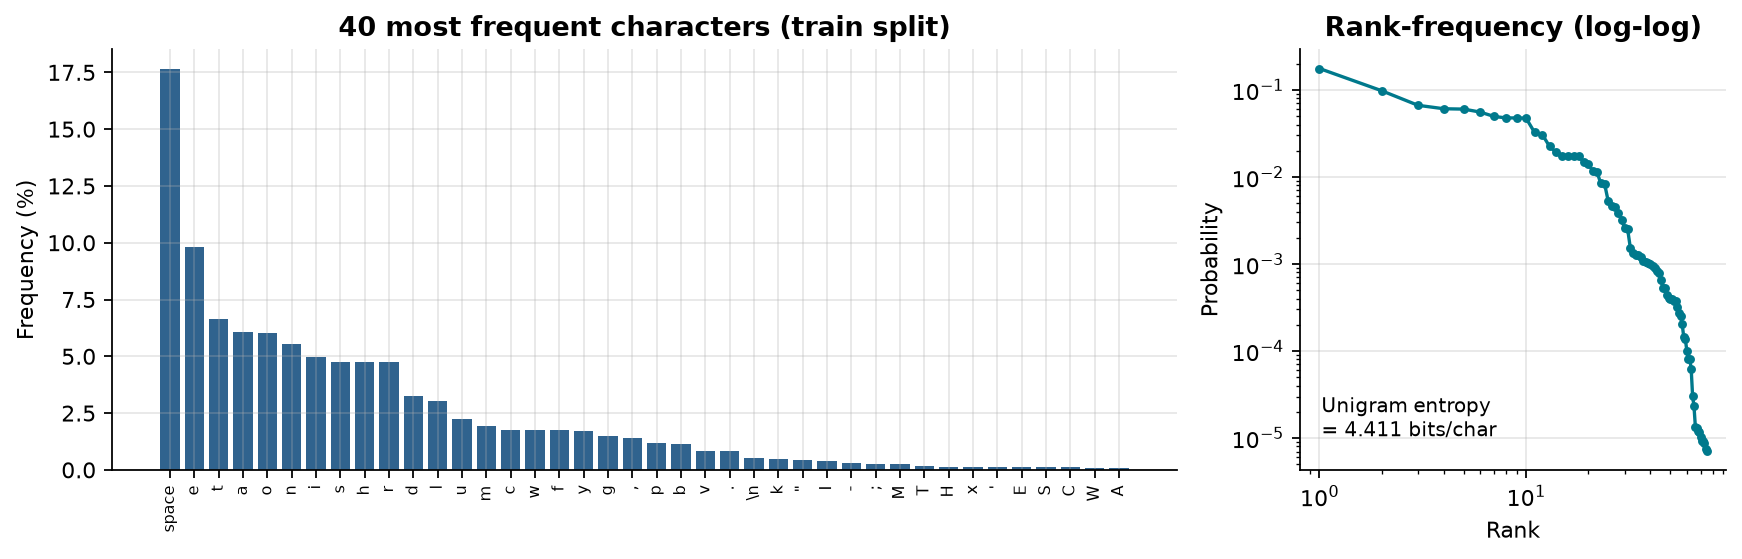
\includegraphics[width=0.92\textwidth]{eda_char_frequency.png}
\caption{Left: the 40 most frequent characters in the training split. Right: rank--frequency plot on log--log axes; the unigram entropy is \unigramH~bits per character.}
\label{fig:charfreq}
\end{figure*}

The most useful statistic for our purposes is sparsity (Fig.~\ref{fig:sparsity}). We measured how many character $n$-grams in the validation text never occur in the 3.6~M-character training text. Up to $n=5$ almost everything has been seen (\unseenfive\% unseen), but the share rises to \unseenseven\% for $n=7$, \unseeneight\% for $n=8$ and \unseenten\% for $n=10$. A count-based model therefore cannot rely on contexts longer than six or seven characters, whereas a recurrent network compresses any history into a dense vector and can generalise to contexts it has never seen. This is the main reason to expect the neural models to win.

\begin{figure}[!t]
\centering
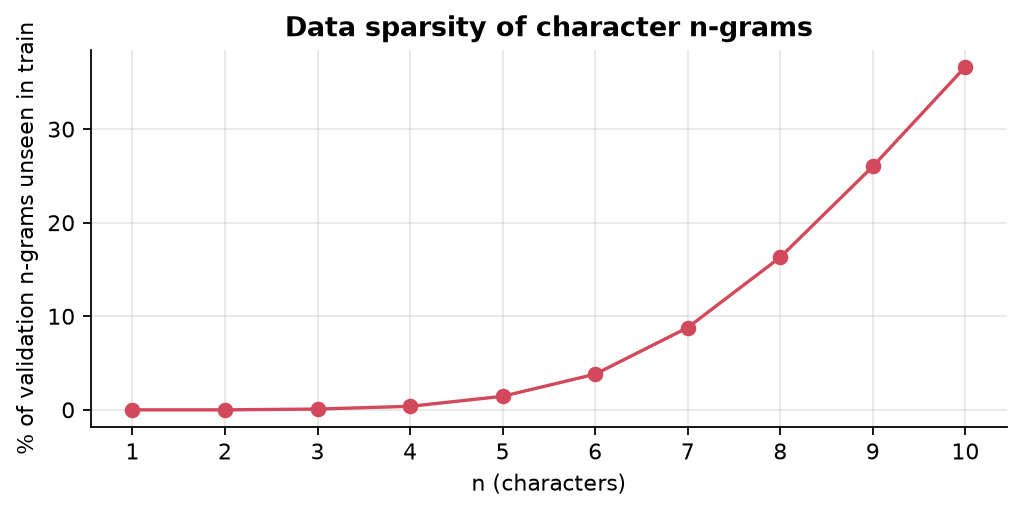
\includegraphics[width=0.95\columnwidth]{eda_ngram_sparsity.png}
\caption{Share of validation character $n$-grams that never appear in the training split.}
\label{fig:sparsity}
\end{figure}

\section{Methodology}
\subsection{Workflow}
Fig.~\ref{fig:workflow} summarises the pipeline. The top row prepares and analyses the data, the middle row is the training and evaluation loop shared by every neural model, and the bottom row lists the experiment groups built on top of it. All runs were executed by a single script on a 16-core Linux server without a GPU.

\begin{figure*}[!t]
\centering
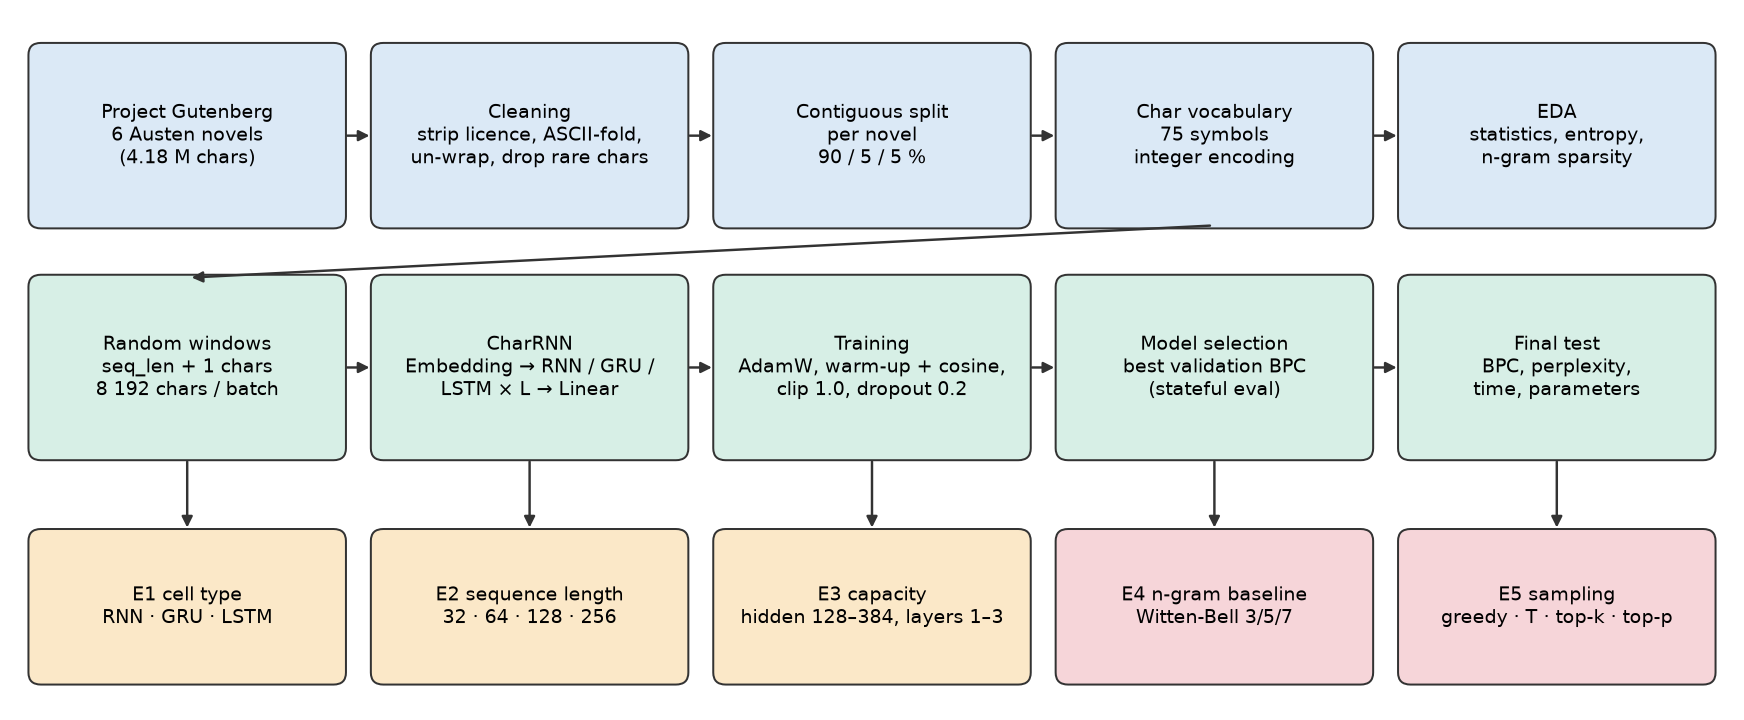
\includegraphics[width=0.95\textwidth]{workflow_diagram.png}
\caption{End-to-end workflow: data preparation (top), the shared training and evaluation loop (middle) and the experiment groups (bottom).}
\label{fig:workflow}
\end{figure*}

\subsection{Model}
Every neural model is an instance of one class (Fig.~\ref{fig:arch}). A 64-dimensional embedding feeds a stack of recurrent layers, dropout is applied to the top hidden state, and a linear layer produces logits over the \vocab~characters. Only the recurrent cell and its size change between runs.

\begin{figure*}[!t]
\centering
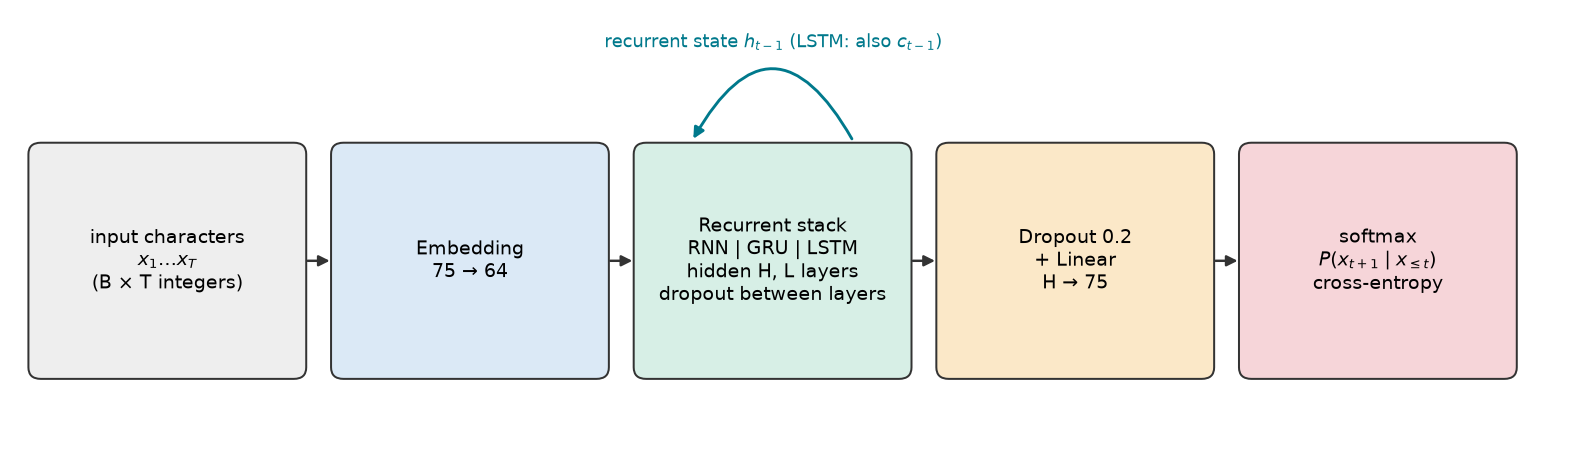
\includegraphics[width=0.85\textwidth]{model_architecture.png}
\caption{The CharRNN architecture. The recurrent state is carried from one step to the next during training and, across 256-character chunks, during evaluation.}
\label{fig:arch}
\end{figure*}

The vanilla RNN updates its state with a single non-linearity,
\begin{equation}
h_t = \tanh(W_x x_t + W_h h_{t-1} + b).
\end{equation}
The GRU adds an update gate $z_t$ and a reset gate $r_t$:
\begin{align}
z_t &= \sigma(W_z x_t + U_z h_{t-1}), \quad r_t = \sigma(W_r x_t + U_r h_{t-1}),\\
\tilde h_t &= \tanh\big(W x_t + U (r_t \odot h_{t-1})\big),\\
h_t &= (1 - z_t)\odot h_{t-1} + z_t \odot \tilde h_t .
\end{align}
The LSTM keeps a separate cell state $c_t$ controlled by input, forget and output gates $i_t, f_t, o_t$:
\begin{align}
c_t &= f_t \odot c_{t-1} + i_t \odot \tanh(W_c x_t + U_c h_{t-1}),\\
h_t &= o_t \odot \tanh(c_t).
\end{align}
The additive update of $c_t$ gives gradients an almost linear path through time~\cite{hochreiter1997lstm}. At equal width the GRU has three weight blocks per layer and the LSTM four, so they carry about 2.8 and 3.7 times the parameters of the vanilla RNN (Table~\ref{tab:params}).

\begin{table}[!t]
\centering
\caption{Parameters at hidden size 256 and two layers.}
\label{tab:params}
\fittable{generated/tab_params.tex}
\end{table}

\subsection{Training}
All models minimise next-character cross-entropy with AdamW~\cite{loshchilov2019} at a peak learning rate of $2\times10^{-3}$, a 100-step linear warm-up and cosine decay to zero. Each run takes 2{,}500 updates of 8{,}192 characters, about 20.5~M characters or 5.6 passes over the training text. Instead of fixing the batch size we fix the number of characters per update, so a model with 32-character windows sees 256 sequences per batch and one with 256-character windows sees 32. This keeps the compute per update equal across sequence lengths. Gradients are clipped at a global norm of 1.0~\cite{pascanu2013}, dropout is 0.2, and the seed is fixed at 42. The model is evaluated on validation text every 250 updates and the best checkpoint is kept.

\subsection{Evaluation}
We report bits per character and character perplexity on held-out text,
\begin{equation}
\BPC = -\frac{1}{N}\sum_{t=1}^{N}\log_2 p(x_t \mid x_{<t}), \qquad \mathrm{PPL} = 2^{\BPC}.
\end{equation}
BPC is the average number of bits an ideal compressor using the model would need per character. Evaluation is \emph{stateful}: the text is split into 32 parallel streams that are read left to right in 256-character chunks while the hidden state is carried forward, so every character is predicted with its full history. This matters for RQ2, because otherwise a model trained on 32-character windows would also be evaluated with at most 32 characters of context.

\subsection{Baseline}
The $n$-gram baseline uses interpolated Witten--Bell smoothing~\cite{witten1991},
\begin{equation}
P_k(c\mid h) = \frac{C(hc) + T(h)\,P_{k-1}(c\mid h')}{C(h) + T(h)},
\end{equation}
where $T(h)$ counts the distinct characters observed after context $h$ and $h'$ drops the oldest character. It needs no tuning and is fitted on exactly the same training text.

\subsection{Experimental design}
E1 compares the three cells (hidden 256, two layers, sequence length 128). E2 trains the LSTM with BPTT windows of 32, 64, 128 and 256. E3 varies the LSTM's hidden size (128, 256, 384) and depth (1, 2, 3 layers). E4 fits $n$-gram models of order 3, 5 and 7. E5 generates text from the best model with seven decoding strategies. Finally, E6 retrains the best configuration for longer to see how far it can go.

\section{Results}
Table~\ref{tab:runs} lists all ten controlled runs. The best model by validation score is highlighted.

\begin{table*}[!t]
\centering
\caption{All controlled runs (2{,}500 updates each). $H$: hidden size, $L$: layers, $T$: BPTT length. Wall-clock times are approximate because three runs shared the CPU.}
\label{tab:runs}
\footnotesize
\begin{tabular}{llrrrrrrrr}
\toprule
Exp. & Cell & $H$ & $L$ & $T$ & Params (M) & Val BPC & Test BPC & Test PPL & Time (min) \\
\midrule
E1 & RNN & 256 & 2 & 128 & 0.238 & 1.791 & 1.766 & 3.401 & 20.5 \\
E1 & GRU & 256 & 2 & 128 & 0.666 & \textbf{1.611} & \textbf{1.585} & 3.000 & 45.4 \\
E1 & LSTM & 256 & 2 & 128 & 0.88 & 1.752 & 1.726 & 3.308 & 36.9 \\
E2 & LSTM & 256 & 2 & 32 & 0.88 & 1.761 & 1.736 & 3.332 & 33.0 \\
E2 & LSTM & 256 & 2 & 64 & 0.88 & 1.757 & 1.731 & 3.320 & 43.2 \\
E2 & LSTM & 256 & 2 & 256 & 0.88 & 1.747 & 1.720 & 3.295 & 56.1 \\
E3 & LSTM & 128 & 2 & 128 & 0.246 & 2.047 & 2.027 & 4.075 & 19.5 \\
E3 & LSTM & 384 & 2 & 128 & 1.908 & 1.623 & 1.599 & 3.030 & 83.6 \\
E3 & LSTM & 256 & 1 & 128 & 0.354 & 1.851 & 1.830 & 3.555 & 25.3 \\
E3 & LSTM & 256 & 3 & 128 & 1.406 & 1.843 & 1.818 & 3.525 & 71.0 \\
\bottomrule
\end{tabular}

\end{table*}

\subsection{E1: cell type}
The GRU is the clear winner of the equal-budget comparison with \tbpcgru~test BPC, against \tbpclstm~for the LSTM and \tbpcrnn~for the vanilla RNN. The learning curves (Fig.~\ref{fig:e1}) explain the ranking. The GRU drops fastest from the first evaluation onward (2.13~BPC after 250 updates, against 2.30 for the RNN and 2.61 for the LSTM) and stays ahead throughout. The LSTM starts slowest, since its four gates and separate cell state need many updates before they carry useful information, but it overtakes the vanilla RNN between updates 1{,}000 and 1{,}250 and keeps improving faster. The vanilla RNN learns local patterns quickly and then flattens out. None of the validation curves had stopped falling at update 2{,}500, so the ranking reflects learning speed under a fixed budget rather than final capacity; the LSTM is known to catch up with much longer training~\cite{chung2014,jozefowicz2015}.

\begin{figure*}[!t]
\centering
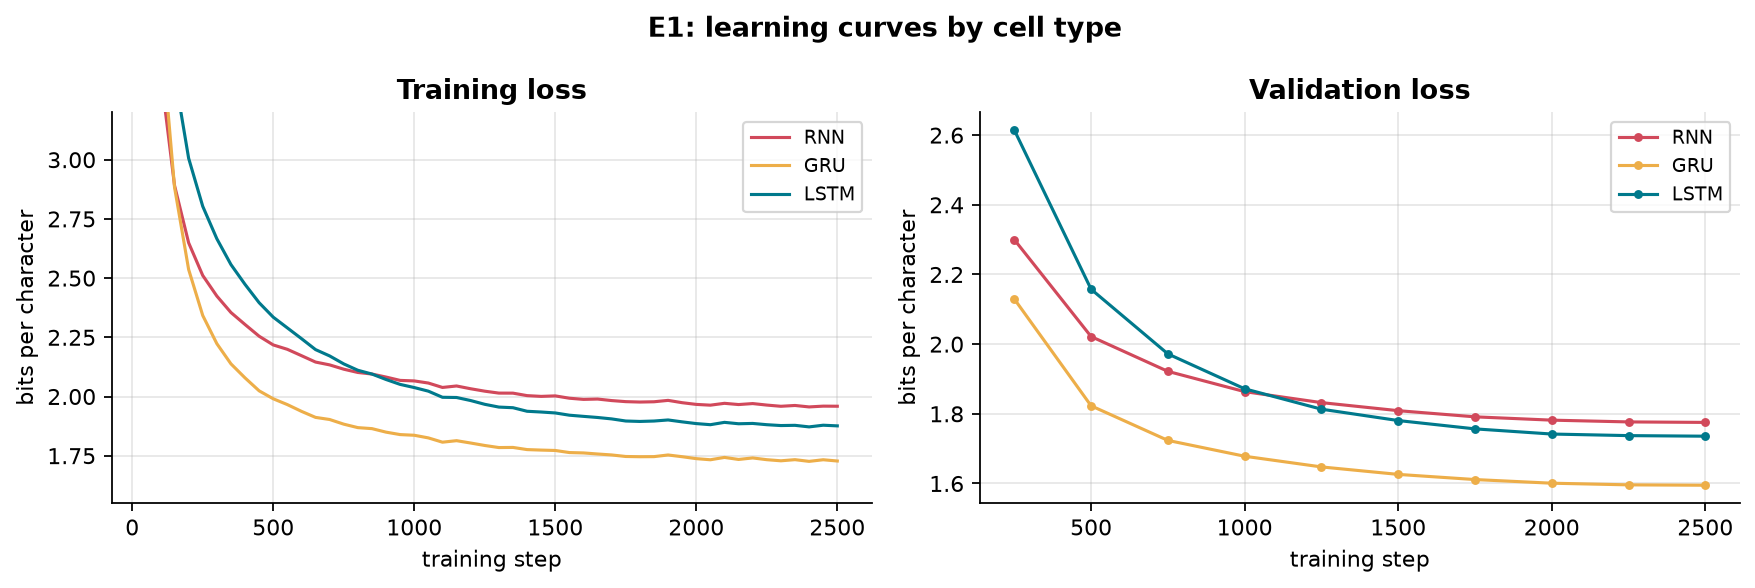
\includegraphics[width=0.92\textwidth]{e1_learning_curves.png}
\caption{E1 learning curves in bits per character: training loss with dropout (left) and validation loss (right).}
\label{fig:e1}
\end{figure*}

We expected the vanilla RNN to suffer from exploding gradients, but it did not. The pre-clipping gradient norm (Fig.~\ref{fig:grad}) peaked at 0.78 and settled between 0.13 and 0.25 for all three cells, so the clipping threshold of 1.0 was never reached. With 128-step windows and a modest learning rate the RNN's weakness lies on the other side of the same problem: vanishing gradients make long-range information hard to learn, which is exactly what gating addresses.

\begin{figure}[!t]
\centering
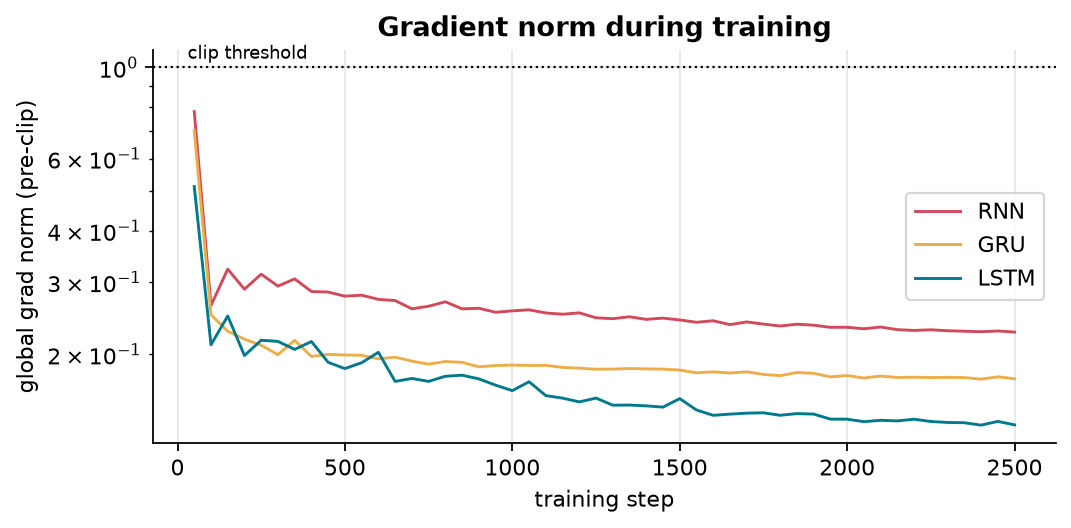
\includegraphics[width=0.95\columnwidth]{e1_grad_norms.png}
\caption{Global gradient norm before clipping (log scale).}
\label{fig:grad}
\end{figure}

\subsection{E2: sequence length}
Longer windows help, but only slightly. Test BPC improves monotonically from \tbpcseqA~(32 characters) to \tbpcseqB~(64), \tbpclstm~(128) and \tbpcseqD~(256), a total gain of less than 0.02~BPC for an eight-fold longer window (Fig.~\ref{fig:e2}). Because evaluation is stateful, even the model trained on 32-character windows uses long histories at test time. What a longer window adds is the ability to \emph{learn} dependencies longer than the window, such as closing a quotation or keeping a name consistent within a sentence. The cost rises noticeably: the 256-character run was the slowest LSTM run (\minseqD~min against \minseqA~min for 32), because fewer, longer sequences per batch parallelise worse. For this corpus 128--256 characters, roughly one sentence, is a sensible choice.

\begin{figure*}[!t]
\centering
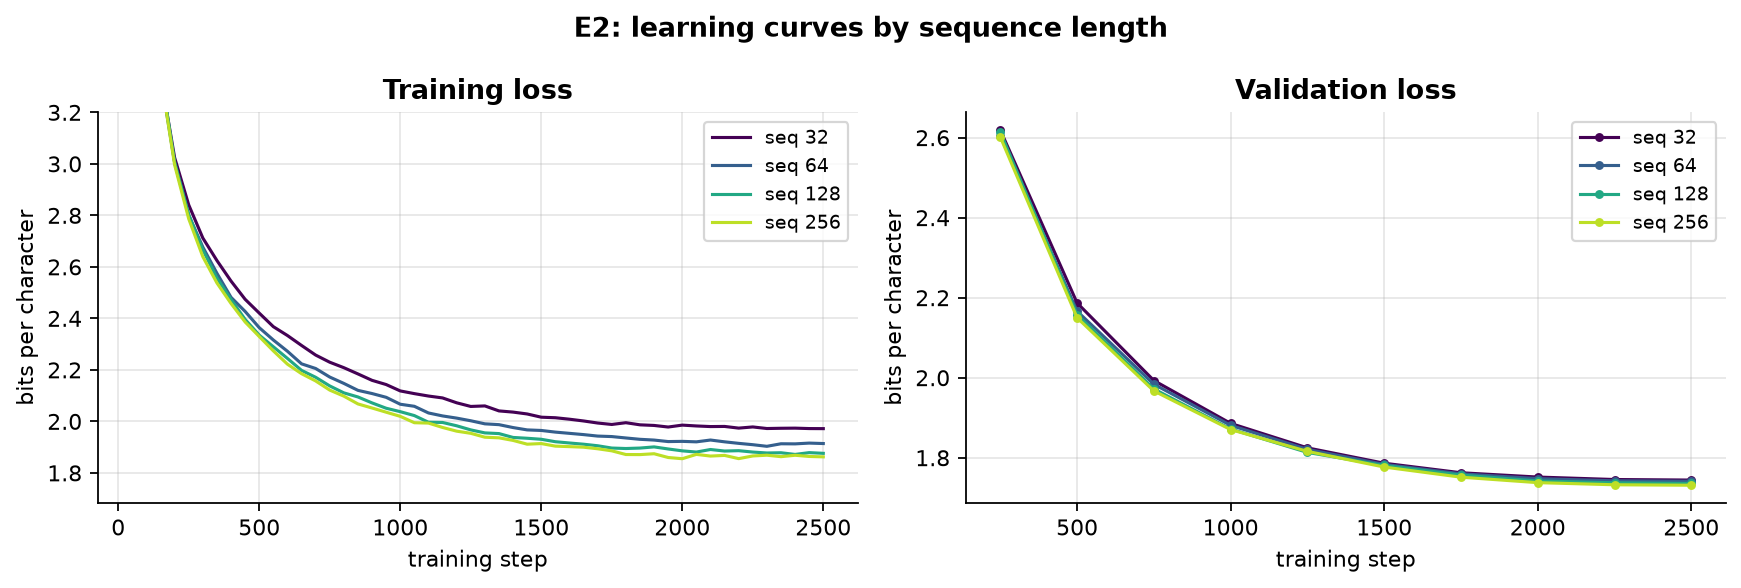
\includegraphics[width=0.92\textwidth]{e2_learning_curves.png}
\caption{E2 learning curves for BPTT windows of 32 to 256 characters.}
\label{fig:e2}
\end{figure*}

\subsection{E3: capacity and depth}
Width matters most. Halving the hidden size to 128 raises the test score to \tbpchsmall~BPC, while 384 units lower it to \tbpchlarge, the largest gain obtained by changing the LSTM (Fig.~\ref{fig:e3}). Wider layers both store more and learn faster per update: after 750 updates the 384-unit model was at 1.80~BPC while the 256-unit model was still at 1.97. Depth helps up to a point. A single layer reaches only \tbpclone~BPC, so the second layer, which can combine character patterns into word-level features, is clearly worthwhile. A third layer does not pay off within the budget: it starts very slowly (3.17~BPC after 250 updates) and ends at \tbpclthree.

\begin{figure*}[!t]
\centering
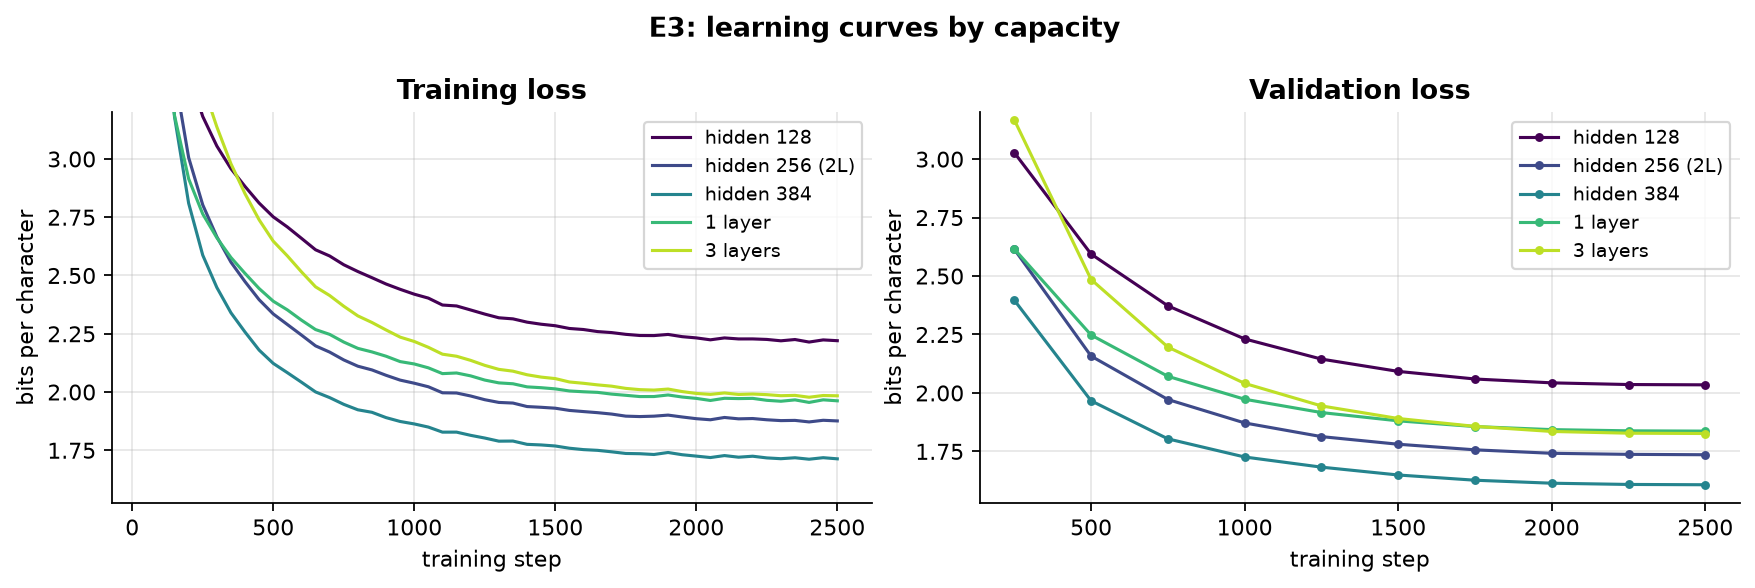
\includegraphics[width=0.92\textwidth]{e3_learning_curves.png}
\caption{E3 learning curves for different hidden sizes and depths of the LSTM.}
\label{fig:e3}
\end{figure*}

The 384-unit LSTM almost catches the GRU (\tbpchlarge~vs \tbpcgru) but needs 2.9 times the parameters and 1.8 times the training time. The E1 result is therefore not simply a matter of size: per parameter and per update, the GRU is the most efficient cell here (Fig.~\ref{fig:tradeoff}).

\begin{figure*}[!t]
\centering
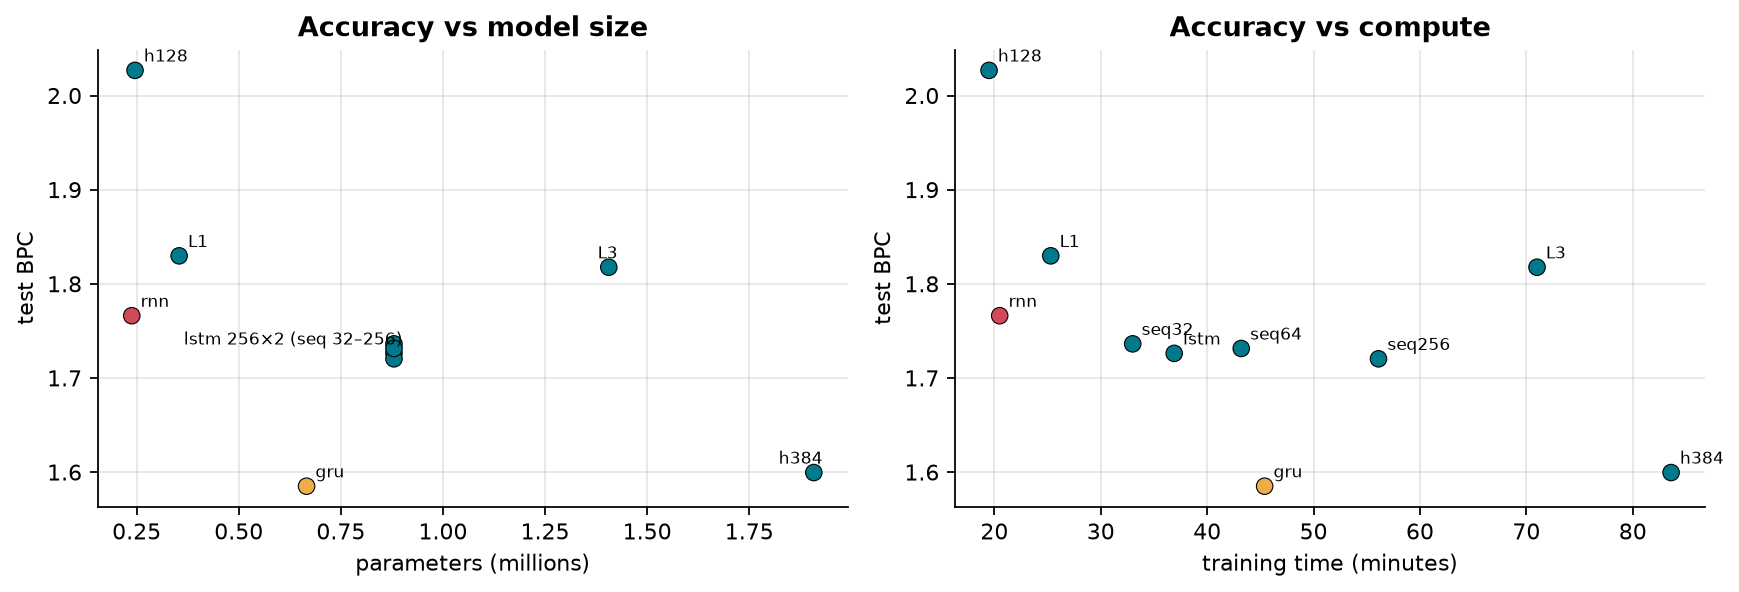
\includegraphics[width=0.85\textwidth]{tradeoff.png}
\caption{Test BPC against parameter count (left) and training time (right). Colour indicates the cell type.}
\label{fig:tradeoff}
\end{figure*}

\subsection{E4: comparison with $n$-gram models}
Table~\ref{tab:baselines} puts the neural results in perspective. The 3-gram is far behind at \ngthree~BPC, but the 5-gram is strong at \ngfive, better than the vanilla RNN and every LSTM except the 384-unit model. Raising the order to 7 makes the $n$-gram \emph{worse} (\ngseven): as the sparsity analysis predicted, most 7-character contexts are seen too rarely to estimate reliably. Under the equal budget the GRU beats the best $n$-gram by \gruvsng\% using \pargru~M parameters, while the 5-gram stores \ngctxfive~thousand distinct contexts and cannot improve further without more data.

\begin{table}[!t]
\centering
\caption{Neural models versus count-based baselines on the same test text.}
\label{tab:baselines}
\fittable{generated/tab_baselines.tex}
\end{table}

\subsection{E5: decoding strategies}
We generated text from the best E1 model for four prompts, three seeds and 800 characters per strategy, and scored it automatically (Table~\ref{tab:sampling}, Fig.~\ref{fig:sampling}). \emph{Valid} is the share of generated words found in the training vocabulary, \emph{Dist-1/2} the share of distinct word unigrams and bigrams, \emph{Rep-4} the share of repeated word 4-grams, and \emph{NLL} the model's own surprise at the sample in BPC.

\begin{table}[!t]
\centering
\caption{Automatic quality of generated text (mean of 12 samples per strategy).}
\label{tab:sampling}
\fittable{generated/tab_sampling.tex}
\end{table}

Greedy decoding degenerates. Always choosing the most likely character produces fluent fragments that loop (``of the same time to be a servant of the same time\ldots''): \greedyrep\% of its word 4-grams are repeats and its Dist-2 is only \greedydtwo. It also has the lowest NLL (\greedynll~BPC), a clear illustration that the most probable sequence is not a good sample~\cite{holtzman2020}. Temperature trades spelling for diversity. At $\tau=0.5$ almost every word is real (\tfivevalid\%) but the vocabulary is narrow (Dist-1 \tfivedone~vs \tonedone~at $\tau=1.0$). At $\tau=1.0$ the valid-word rate falls to \tonevalid\%, and at $\tau=1.3$ to \thirteenvalid\%, with many invented words. Truncated sampling gives the best compromise: nucleus sampling with $p=0.9$ keeps \nucvalid\% valid words with a Dist-2 of \nucdtwo~and no repeated 4-grams. Its samples have correct punctuation, dialogue formatting and period vocabulary, but little coherence beyond a sentence or two.

\begin{figure*}[!t]
\centering
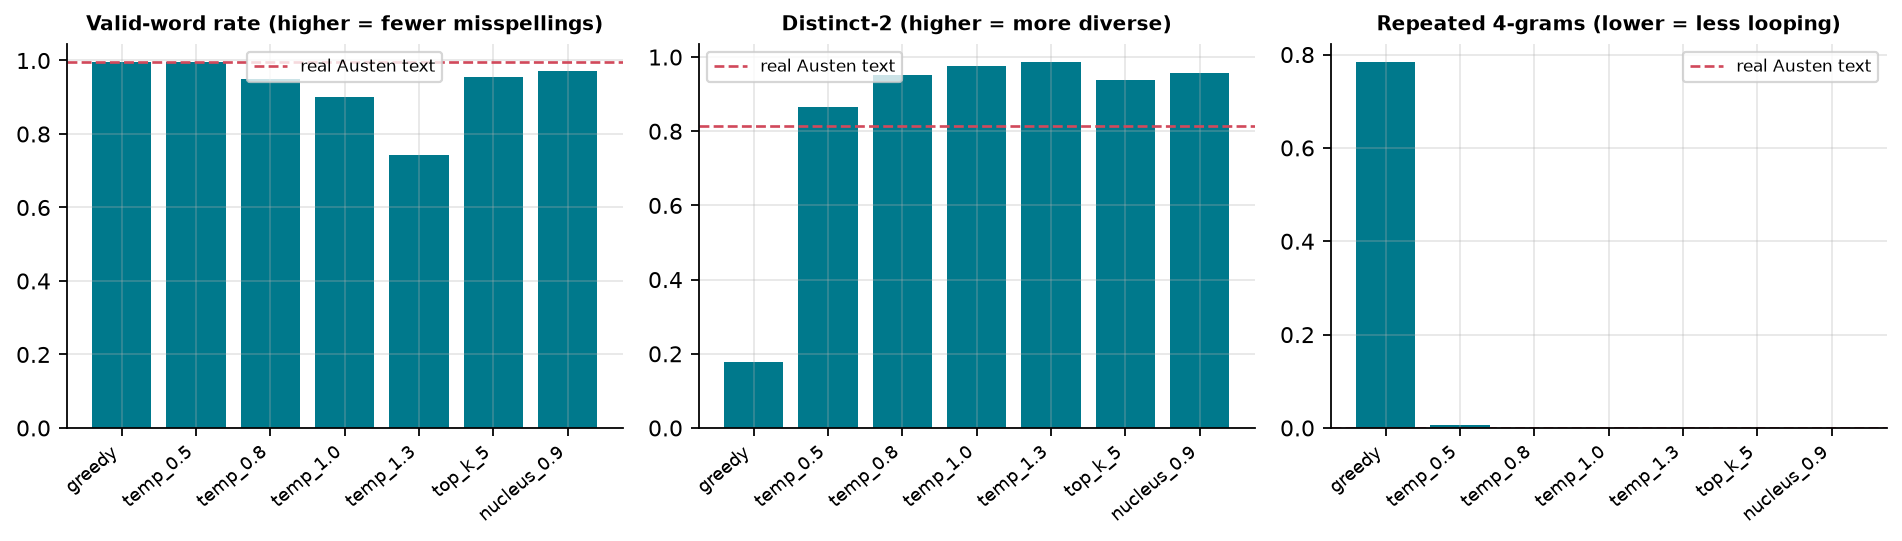
\includegraphics[width=0.92\textwidth]{e5_sampling_metrics.png}
\caption{Spelling quality, diversity and repetition for each decoding strategy. The dashed line marks real held-out text.}
\label{fig:sampling}
\end{figure*}

\subsection{E6: training the best model longer}
E1--E5 compare models under an equal budget. E6 asks a different question: how good does the winning configuration get when it is simply trained longer? We retrained the GRU ($256\times2$, $T=128$) for \finsteps~updates, \finratio~times the original budget or about \finepochs~passes over the training text, with everything else unchanged. It reaches \textbf{\bestbpc~BPC} on the test set (perplexity \bestppl), \fingain~BPC better than the 2{,}500-update run and \finvsng\% better than the best $n$-gram. The validation curve (Fig.~\ref{fig:e6}) falls throughout, which confirms that every model in the controlled study was limited by compute rather than by data or capacity.

\begin{figure}[!t]
\centering
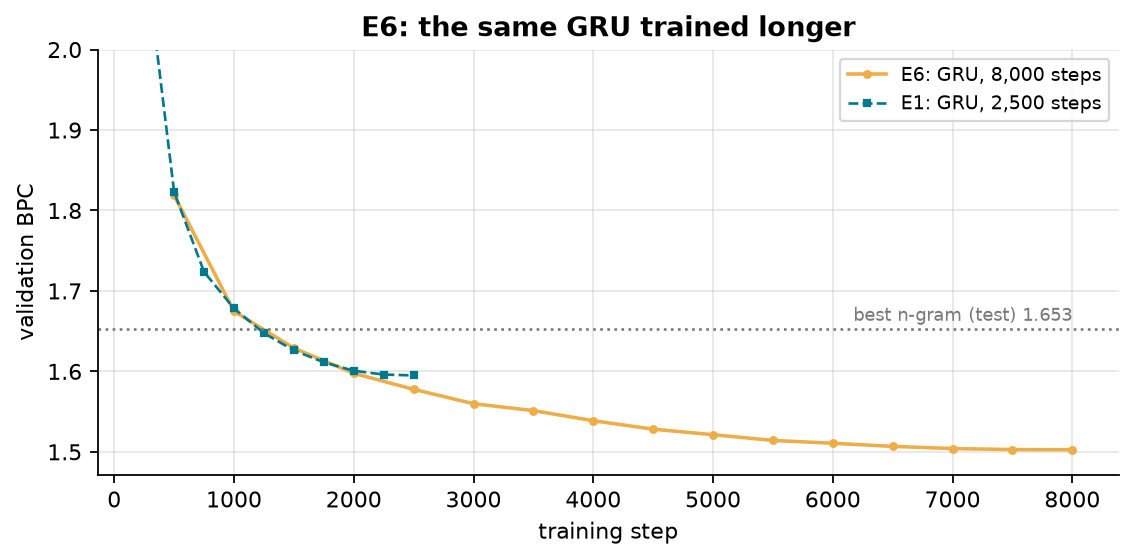
\includegraphics[width=0.95\columnwidth]{e6_final_model.png}
\caption{Validation BPC of the GRU trained for \finsteps~updates (E6) compared with the 2{,}500-update run of E1. The dotted line is the best $n$-gram test score.}
\label{fig:e6}
\end{figure}

This run also taught us something practical. On our 16-core CPU the small GRU trained fastest with only two threads (0.64~s per update) and five times slower with twelve (3.1~s), because its matrices are too small for multi-threading to pay off and the threads mostly wait on each other. A one-minute benchmark turned a run that would have taken about seven hours into one of \finmin~minutes.

\subsection{What did the network learn?}
To see what the model represents, we ran the best E1 GRU over \interpchars~characters of test text, recorded its 256 top-layer hidden units at every step, and related them to six properties of the text. For each property we report the most correlated single unit, following Karpathy~\textit{et~al.}~\cite{karpathy2015}, and a linear probe~\cite{alain2016probes} trained on 70\% of the characters and tested on the remaining 30\%. As a control, an identical probe sees only the \emph{current} character. If the hidden-state probe does clearly better, the network must be storing information about the past (Table~\ref{tab:probes}).

\begin{table}[!t]
\centering
\caption{Linear probes on the GRU hidden state (\emph{Hidden}) versus the current character only (\emph{Char}); \emph{Base} is the majority class.}
\label{tab:probes}
\fittable{generated/tab_probes.tex}
\end{table}

A quotation detector emerged without any supervision. Unit~\qunit~correlates with being inside a quotation at $|r|=\qr$ (Fig.~\ref{fig:units}, top): its activation changes at an opening quotation mark, holds through the whole speech, briefly relaxes during the narrator's interruption ``replied Darcy,'' and returns to its resting value when the quotation closes. A probe on the hidden state predicts whether the text is inside a quotation with \qacc\% accuracy; the current character alone gives \qacccur\%, no better than the majority class (\qmaj\%). Nobody told the model what a quotation is. It learned to keep track of one because closing quotations correctly lowers the loss.

\begin{figure*}[!t]
\centering
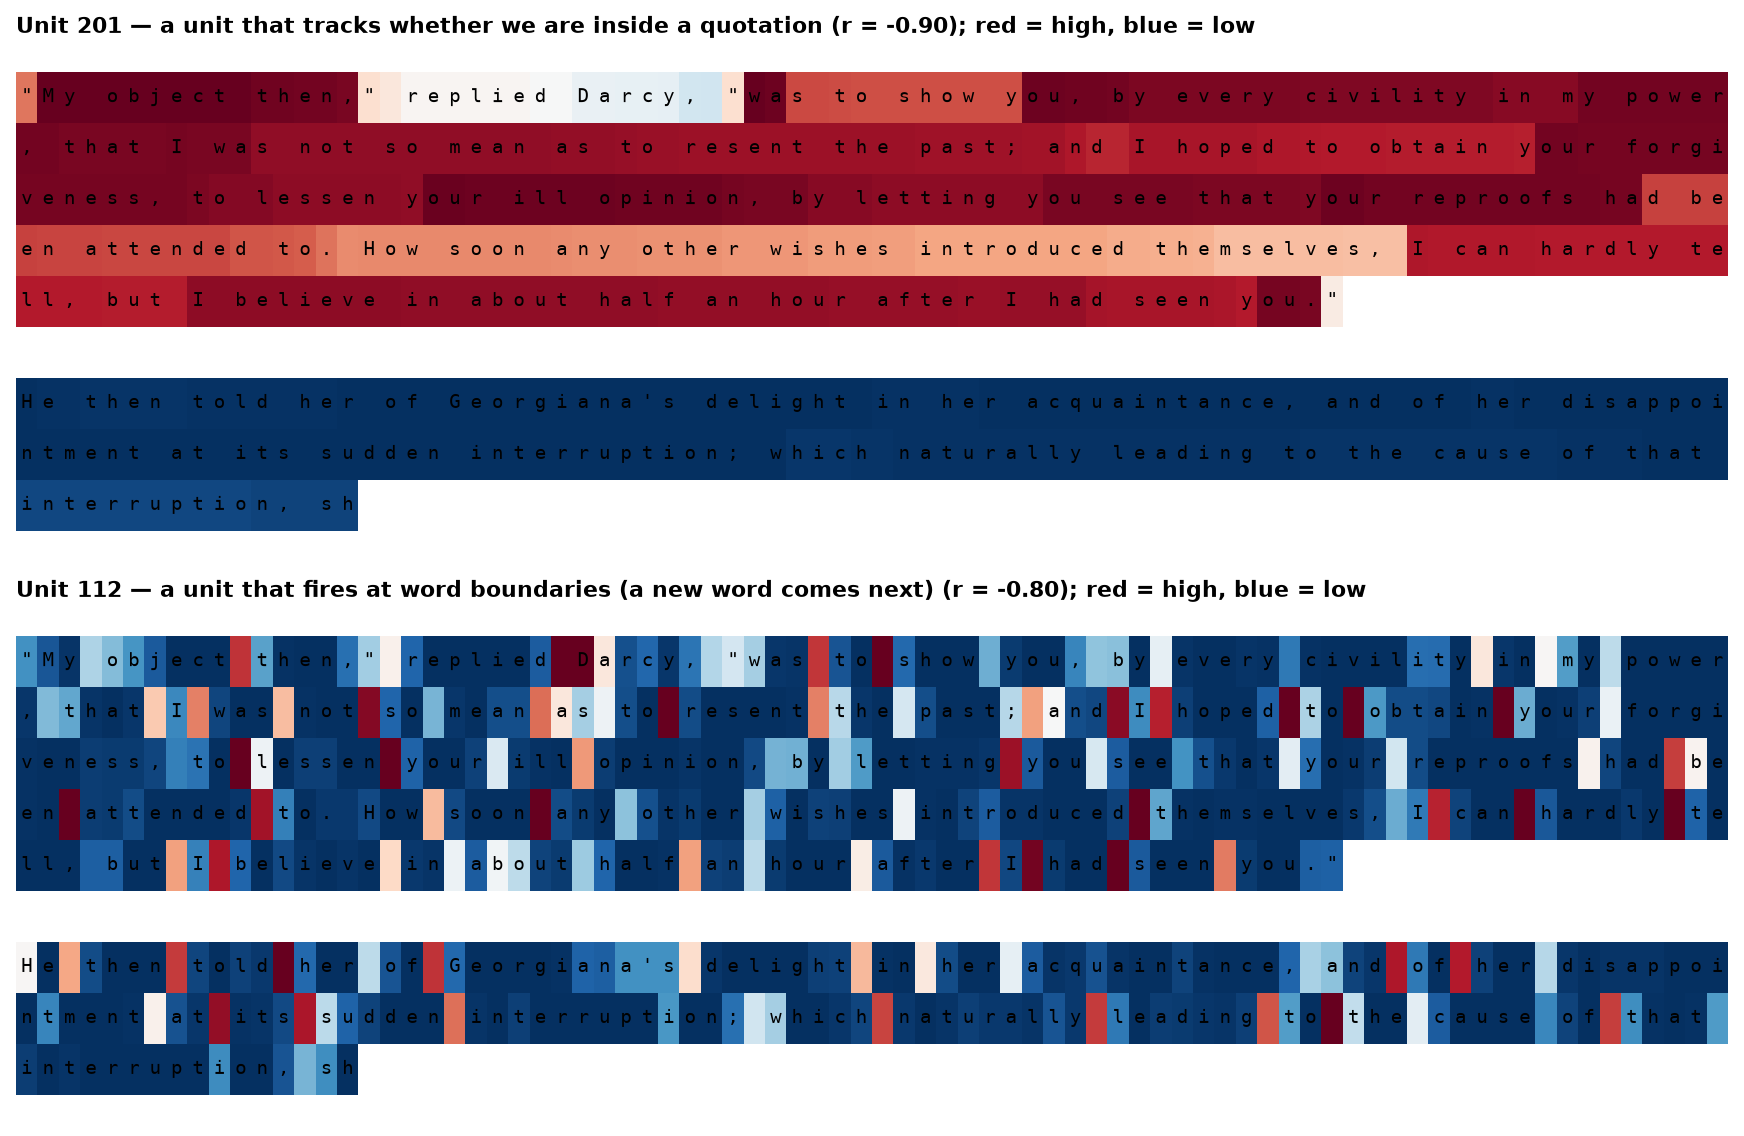
\includegraphics[width=0.9\textwidth]{interp_unit_activations.png}
\caption{Activation of two hidden units over a passage of \textit{Pride and Prejudice} from the test split (red: high, blue: low). Top: unit \qunit, which tracks quotations. Bottom: unit \bunit, which fires at word boundaries.}
\label{fig:units}
\end{figure*}

Word structure is tracked too. Unit~\bunit~fires at word boundaries ($|r|=\br$), and the position inside the current word can be read from the hidden state with $R^2=\wordrtwo$, against \wordrtwocur~from the current character. Capital letters and sentence ends, in contrast, are already given by the current character, so the hidden state adds nothing for them. The position within a long paragraph is not represented at all, which fits the 128-character training windows: the model never had a reason to count beyond about one sentence.

\subsection{Interactive demo}
To make the result tangible we exported the final GRU to a 1.8~MB JavaScript file (float16 weights) and re-implemented the GRU cell in about a hundred lines of plain JavaScript. The page (Fig.~\ref{fig:demo}) runs entirely in the browser without a server. It lets the user choose a prompt, a decoding strategy and its parameters, and streams several hundred characters per second. Its logits match PyTorch to within $3\times10^{-6}$, and its greedy output matches the Python implementation character for character.

\begin{figure}[!t]
\centering
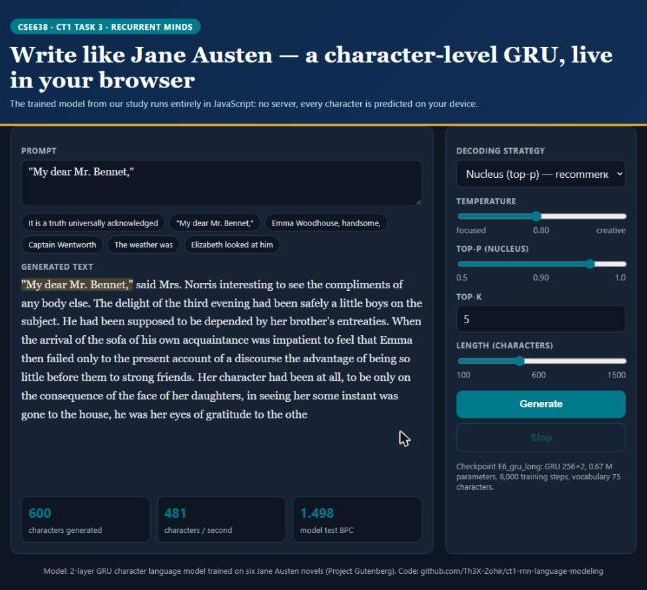
\includegraphics[width=0.92\columnwidth]{demo_screenshot.png}
\caption{The browser demo generating text from the prompt ``My dear Mr.~Bennet,'' with nucleus sampling, using the E6 model.}
\label{fig:demo}
\end{figure}

\section{Discussion}
\textit{Why does the GRU win?} Under a short budget the GRU combines the benefit of gating with a simpler structure than the LSTM: two gates instead of three and no separate cell state, so fewer parameters have to co-adapt before the model becomes useful. This matches earlier reports~\cite{chung2014,jozefowicz2015}, and we read our result as ``the GRU is the most efficient cell for a small compute budget'' rather than as a universal ranking.

\textit{What matters most?} Ordered by effect size, the levers were the hidden size (0.43~BPC between 128 and 384 units), the cell type (0.18~BPC between the RNN and the GRU), depth (0.10~BPC between one and two layers) and, a distant last, the BPTT window (0.02~BPC between 32 and 256 characters). Training time, in turn, was worth almost as much as any architectural change (0.09~BPC in E6).

\textit{Why is training loss higher than validation loss?} In every run the training BPC is above the validation BPC. This is expected rather than a bug: training loss is measured with dropout active and on random windows whose first characters have no history, whereas evaluation runs without dropout and with the full carried-over state. Together with validation curves that never turned upward, it shows that no model over-fitted.

\textit{Recommendation.} For character-level modeling on a CPU budget, a two-layer GRU with 256 units and a 128--256-character window is a good default. Extra compute is best spent on width and on longer training rather than on depth or longer windows. For generation, nucleus sampling with $p\approx0.9$ or a temperature around 0.8 should replace greedy decoding.

\section{Limitations and Future Work}
Each controlled configuration was trained once with a fixed seed, so differences of a few thousandths of a BPC are within run-to-run noise; the large effects are well above it. The controlled budget is short, and larger models in particular were still improving when it ended. E1 compares cells at equal width rather than equal parameter count, although E3 shows that size alone does not explain the gap. The corpus is a single author's 19th-century prose, so absolute numbers do not transfer to other domains. Finally, the generation study relies on automatic proxies that capture spelling, diversity and repetition but not coherence or style.

Natural next steps are: repeating every configuration with several seeds and reporting confidence intervals; comparing against a character-level Transformer with the same parameter budget; adding layer normalisation and weight tying to the long-training run; testing sub-word tokenisation; and running a small blind human evaluation of generated passages.

\section{Conclusion}
We built a reproducible pipeline for character-level language modeling on six Jane Austen novels and used it to compare recurrent architectures under a controlled budget. The two-layer GRU learned fastest and reached \tbpcgru~BPC under the equal budget and \bestbpc~BPC when trained longer, beating every LSTM configuration, the vanilla RNN and a strong Witten--Bell 5-gram. Width, gating and training time mattered far more than the BPTT window. Inside the trained network we found a unit that tracks quotations and a linearly decodable sense of word position, and the final model runs live in a browser.

\section*{Code and Data Availability}
The complete code base (data pipeline, models, training and evaluation scripts, interpretability analysis, browser demo, unit tests, executed notebook and all trained checkpoints) is available at \url{https://github.com/Th3X-Zohir/ct1-rnn-language-modeling}. The corpus is public-domain text from Project Gutenberg (book IDs 1342, 158, 161, 141, 121 and 105) and is downloaded automatically by the pipeline.

\section*{Declaration of AI Use}
An AI coding assistant was used to help write and debug parts of the code and to format this report. All experiments were run by the authors, every number in this paper is produced by the code in the repository, and all authors reviewed the implementation and the text.

\bibliographystyle{IEEEtran}
\bibliography{references}

\end{document}
